\chapter{Cheatsheet}%

\section{HTML}%
\label{sec:html}

\subsection{Structuur}%
\label{sub:structuur}

Elk \HTML bestand begint met volgende tekst. Dit vertelt de computer dat we \HTML willen gebruiken en geeft extra informatie over hoe de computer onze website moet weergeven.
\inputminted{html}{../cheatsheet/basis_html.html}

\HTML bestaat uit tags. Een tag komt in 2 vormen voor:
\begin{itemize}
    \item Met een begin en een eind die inhoud bevat:
        \begin{minted}{html}
<div>inhoud van de tag</div>
        \end{minted}
    \item Zonder inhoud:
        \begin{minted}{html}
<input />
        \end{minted}
\end{itemize}

Elke tag kan ook extra informatie bevatten via attributen. Deze zijn vaak optioneel maar handig.

\begin{itemize}
    \item Met een begin en een eind die inhoud bevat:
        \begin{minted}{html}
<div id="mijn_id" class="mijn_klasse">
    inhoud van de tag
</div>
        \end{minted}
    \item Zonder inhoud:
        \begin{minted}{html}
<input id="mijn_id" type="password" />
        \end{minted}
\end{itemize}

\Opm \HTML houd geen rekening met spaties, tabs, ... Dus volgende 2 notaties zijn hetzelfde:
\begin{minted}{html}
<div
    class="blabla"
    id="blabla">
        Dit is indoud
</div>
<div class="blabla" id="blabla">Dit is indoud</div>
<div class="blabla" id="blabla">Dit is indoud met veel spaties
                        </div>
\end{minted}

\subsection{Voorbeeld rood vierkant}%
\label{sub:voorbeeld_rood_vierkant}

Plaatsen van een rood vierkant op een gekozen locatie:
\inputminted{html}{../cheatsheet/pos_div.html}

Het grote verschil met de begincode is de \textbf{div}. En deze heeft 1 groot attribuut \textbf{style}. De waarde hierin is eigenlijk \CSS waarover later meer.

Kort overlopen van de verschillende waarden in de \textbf{style}:
\begin{itemize}
    \item \emph{background}: achtergrond rood (red) maken
    \item \emph{width}: breedte op \emph{100px} zetten
    \item \emph{height}: hoogte op \emph{100px} zetten
    \item \emph{position}: nodig om een niet standaard positie te kunnen opgeven
    \item \emph{left}: afstand van de linker rand
    \item \emph{right}: afstand van de top
\end{itemize}

\begin{figure}[htpb]
    \centering
    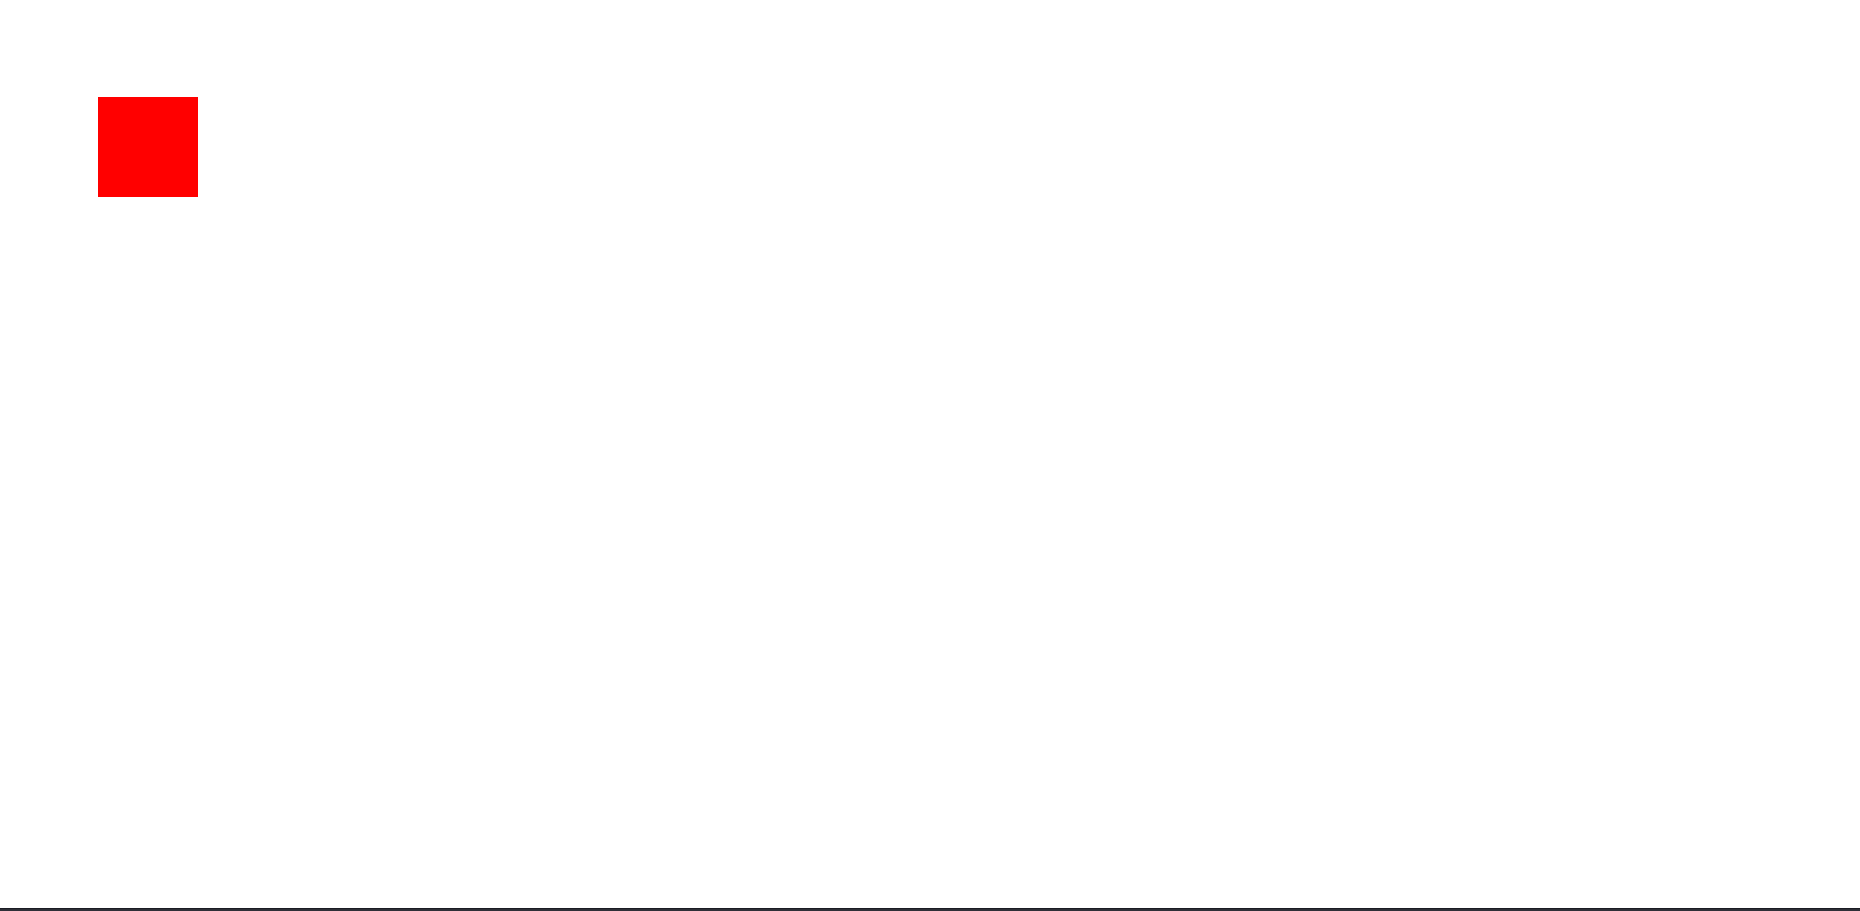
\includegraphics[width=0.6\linewidth]{figures/resultaat_rood_vierkant.png}
    \caption{Resultaat rood vierkant}
    \label{fig:resultaat_rood_vierkant}
\end{figure}

\subsection{Belangrijke HTML tags}%
\label{sub:belangrijke_html_tags}

\begin{itemize}
    \item \emph{html}: Bevat alle andere \HTML tags
    \item \emph{head}: Normaal nooit zichtbaar, maar bevat belangrijke informatie over de \HTML
    \item \emph{body}: Alles in deze tag is zichtbaar op het scherm
    \item \emph{title}: De titel van je website en komt enkel voor in een \emph{head}-tag
    \item \emph{div}: Een block-container zonder extra betekenis
    \item \emph{img}: Voeg een afbeelding toe met de \emph{src}-attribuut (url)
    \item \emph{input}: Tekstveld, handig voor vragen van een spelersnaam
    \item \emph{style}: \CSS voor gans de webpagina
    \item \emph{script}: \JS voor de webpagina
\end{itemize}

\subsection{Belangrijke attributen}%
\label{sub:belangrijke_attributen}

\begin{itemize}
    \item \emph{style}: Voeg \CSS toe direct in de \HTML
    \item \emph{id}: Speciale naam voor de tag (moet uniek zijn voor elke tag)
    \item \emph{class}: Zelfde als \emph{id} maar moet niet uniek zijn
    \item \emph{src} (enkel \emph{img}): De url van de tonen afbeelding
    \item \emph{value} (enkel \emph{input}): De ingevulde waarde in het tekstveld
    \item \emph{type} (enkel \emph{input}): Soort input. Belangrijke mogelijke waarden:
        \begin{itemize}
            \item \emph{text} (Standaard waarde): normale tekst
            \item \emph{password}: wachtwoord
            \item \emph{number}: getal
        \end{itemize}
\end{itemize}

\section{CSS}%
\label{sec:css}

\subsection{Structuur}%
\label{sub:structuur}

\begin{minted}{css}
selector {
    eigenschap: waarde;
}
\end{minted}

Er zijn 2 manieren om \CSS toe te voegen. Ofwel via een \emph{style}-tag in de \emph{head}-tag:
\begin{minted}{html}
...
<head>
    ...
    <style>
        selector1 {
            eigenschap: waarde;
        }
        selector2 {
            eigenschap: waarde;
        }
        selector3 {
            eigenschap: waarde;
        }
    </style>
</head>
...
\end{minted}

Een andere manier is zoals eerder met de \emph{style}-attributen. Het grote verschil is dat er nu geen nood meer is aan de selector:
\begin{minted}{html}
...
<div style="
    eigenschap1: waarde;
    eigenschap2: waarde;
    eigenschap3: waarde;
" ></div>
...
\end{minted}

Een selector is een manier om een aantal tags te selecteren en daarvan de
eigenschappen te wijzigen. Er zijn 3 grote manieren van selecteren:
\begin{itemize}
    \item Via tagnaam: bv: \textbf{div}: selecteert alle divs.
    \item Via classmaam: bv: \textbf{.klasse}: selecteert alle tags die
        \mintinline{html}|class="klasse"| hebben
    \item Via id: bv: \mintinline{css}|#id_naam|: selecteert de tag die
        \mintinline{html}|id="id_naam"| heeft. Dit is normaal altijd 1 tag.
\end{itemize}

\subsection{Interessante eigenschappen}%
\label{sub:interessante_eigenschappen}

Hier is een lijstje van de meest interessante eigenschappen voor het opmaken met
CSS. Alle eigenschappen veranderen iets van alleen de geselecteerde elementen!
\begin{itemize}
    \item \textbf{background}: bepaalt de achtergrond
    \item \textbf{color}: bepaalt de tekstkleur
    \item \textbf{width}: bepaalt de breedte
    \item \textbf{height}: bepaalt de hoogte
    \item \textbf{position}: bepaalt de manier waarop de positie van het
        element wordt bepaalt. De belangrijkste zijn:
        \begin{itemize}
            \item \textbf{absolute}: positie ten opzichte van de linker bovenhoek
            \item \textbf{relative}: positie ten opzichte van de linker
                bovenhoek van de ouder (parent)
            \item \textbf{fixed}: zoals absolute maar wanneer je scrolt, blijft
                het element op zijn plaats
        \end{itemize}
    \item \textbf{left}: afstand van links
    \item \textbf{top}: afstand van de bovenkant
    \item \textbf{right}: afstand van rechts
    \item \textbf{bottom}: afstand van de onderkant
    \item \textbf{margin-\{left,top,right,bottom\}}: minimale afstand van
        links,boven,rechts,onder
    \item \textbf{padding-\{left,top,right,bottom\}}: minimale interne afstand
        van links,boven,rechts,onder
    \item \textbf{opacity}: doorzichtbaarheid
\end{itemize}

De waarden die je in bovenstaande eigenschappen kunt invullen, worden hieronder
opgelijst:
\begin{itemize}
    \item \textbf{Afstand}: px (pixels), \% (procent van de ouder)
    \item \textbf{Kleur}: 
        \begin{itemize}
            \item \textbf{Kleurnaam}: red (rood), green (groen), blue (blauw),
                black (zwart), white (wit)
            \item \textbf{rgb(0-255, 0-255, 0-255)}: Kleur samenstellen uit
                r(ood), g(roen) en b(lauw)
            \item \textbf{hsl(hue, saturation, lightness)}: Kleur samenstellen uit
                hue (tint), saturation (verzadiging), lightness (lichtheid)
            \item \textbf{\#XXXXXX}: Hetzelfde als rgb maar korter. Elke kleur 
                bestaat uit 2 tekens tussen 0-9+A-F. Enkele voorbeelden:
                \begin{itemize}
                    \item Wit: \#FFFFFF
                    \item Zwart: \#000000
                    \item Rood: \#FF0000
                    \item Groen: \#00FF00
                    \item Blauw: \#0000FF
                \end{itemize}
        \end{itemize}
\end{itemize}

\section{JavaScript}%
\label{sec:javascript}

\subsection{Structuur}%
\label{sub:structuur}

Om JavaScript de kunnen gebruiken, moet je deze in de HTML in een
\textbf{script}-tag zetten
\begin{minted}{html}
<script type="text/javascript">
    // Dit is een comment
    // Ik wordt nooit uitgevoerd, maar ben hier
    // om jou te helpen
    // In deze tag komt verder alle JavaScript
    console.log("Kijk ik ben cool, druk F12 om mij te zien!");
</script>
\end{minted}

De meest algemene structuur die te vinden is in JavaScript is het
\textbf{statement} 
\begin{minted}{javascript}
console.log("Een beetje veel tekst :)");
\end{minted}
Een aantal dingen om op te merken:
\begin{itemize}
    \item Elke statement bevat een actie (iets doen)
    \item Elke statement eindigt met een punt komma \textbf{;} 
\end{itemize}

Je kunt een statement zien als 1 blokje in Scratch en veel statement na elkaar
is alsof je veel blokjes aan elkaar kunt vastmaken.

\subsubsection{Variabelen}%
\label{ssub:Variabelen}

In Scratch kun je ook variabelen maken. Dit waren stukjes geheugen waar je een 
waarde aan kon meegeven en zo een score kon bijhouden. In JavaScript doe je dit
zo:
\begin{minted}{javascript}
let naamVariabele = 1;
naamVariabele = naamVariabele + 1;
\end{minted}
Een variabele aanmaken begint altijd met het woordje \textbf{let}. Hiermee zeg
je tegen je computer dat hij een stukje geheugen moet reserveren en dat de naam
\textbf{naamVariabele} moet geven.

\Opm Je kunt maar 1 keer een variabele aanvragen onder dezelfde naam in
dezelfde scope (hierover later meer)! Anders gaat de computer klagen. Het is
alsof je in een restaurant 2 reserveringen maakt onder  dezelfde naam. Als je
dan toekomt en ze vragen naar je naam, weten zij niet meer welke reservatie
precies voor wie was.

Nu je een variabele hebt, kun je iedere keer je de waarde die je erin hebt
opgeslagen, nodig hebt, gewoon de naam van de variabele gebruiken.

Met het \textbf{=}-symbool zeg je wat er in de variabele moet worden opgeslagen.
Je kunt dus ook de originele waarde terug veranderen. Dit is wat er gebeurt op
de 2de lijn. Eerst wordt \textbf{mijnVariabele} opgeteld bij 1 en wordt het
resultaat opgeslagen in \textbf{mijnVariabele} (mijnVariabele is nu 2).

Soorten waarden dat je kunt opslaan in een variabele:
\begin{itemize}
    \item \mintinline{javascript}|number| (nummer/getal): Vb 1,2,3, 1.234, -4,
        ...
    \item \mintinline{javascript}|string| (tekenreeks of tekst):
        \mintinline{javascript}|"Dit is een string"|
    \item \mintinline{javascript}|bool| (waar of niet waar): Kan slechts 2 waarden bevatten: \mintinline{javascript}|true, false|.
    \item \mintinline{javascript}|array| (lijst): Lijst van waarden: Vb: lijst
        van nummers: \mintinline{javascript}|[1,2,3,4]|.
    \item \mintinline{javascript}|object| (object): Alles wat je niet kunt
        beschrijver als een nummer of stuk tekst (Vb
        \mintinline{javascript}|document,window,console|)
    \item \mintinline{javascript}|null,undefined| (niets, ongedefinieerd):
        opslaan van dingen die je niet kunt opslaan of nog niet weet.
\end{itemize}

\subsubsection{Conditioneel code uitvoeren}%
\label{ssub:Conditioneel code uitvoeren}

Algemene structuur:
\begin{minted}{javascript}
if (testbool) {
    // uit to voeren als true
} else {
    // code uit te voeren als false
}
\end{minted}

Als 1 kleiner is dat 2, print dan naar de console:
\begin{minted}{javascript}
if (1 < 2) {
    console.log("1 is kleiner dan 2");
} else {
    console.log("1 is niet kleiner dan 2");
}
\end{minted}

Je hoeft else niet altijd toe te voegen (optioneel):
\begin{minted}{javascript}
if (1 < 2) {
    console.log("1 is kleiner dan 2");
}
console.log("Ik wordt altijd uitgevoerd");
\end{minted}

Je kunt ook met variabelen werken:
\begin{minted}{javascript}
let i = 1;
if (i < 2) {
    console.log("i is kleiner dan 2");
}
i = 3;
if (i < 2) {
    // Wordt niet uitgevoerd
    console.log("i is kleiner dan 2");
} else {
    console.log("i is niet kleiner dan 2");
}
\end{minted}

\subsubsection{Code herhalen}%
\label{ssub:Code herhalen}

Structuur for i:
\begin{minted}{javascript}
for (let i = 0; i < 10; i++) {
    console.log(i);
}
// Uitvoer:
// 0
// 1
// 2
// 3
// 4
// 5
// 6
// 7
// 8
// 9
\end{minted}

Structuur for of
\begin{minted}{javascript}
let mijnLijst = [1,2,3,4];
for (let nummer of mijnLijst) {
    console.log(nummer);
}
// Uitvoer:
// 1
// 2
// 3
// 4
\end{minted}

Structuur while: zolang de conditie waar is, blijf herhalen
\begin{minted}{javascript}
let i = 10;
while (i > 5) {
    console.log(i);
    i = i - 1;
}
// Uitvoer:
// 10
// 9
// 8
// 7
// 6
\end{minted}

\subsubsection{Groeperen van code}%
\label{ssub:Groeperen van code}

Met de vorige stukken is het nu al mogelijk om al heel complexe programma's te
schrijven. Dit is ook hoe de eerste computers werden geprogrammeerd. Dit leidde 
echter tot het probleem dat code niet hergebruikt kon worden of het moeilijk 
werd voor een mens om het programma logisch nog te begrijpen.

Als antwoord hierop, werden functies (\mintinline{javascript}|function|)
uitgevonden. Dit is een stuk code dat je een naam geeft, optioneel een aantal
parameters en optioneel ook een variabele kan teruggeven. Deze functie kun je
dan overal hergebruiken als je de naam kent.

Structuur van een functie:
\begin{minted}{javascript}
function naamFunctie(parameter1, parameter2) {
    // Doe iets cool met parameter1 en parameter2
    let ietsCool = 1 + 1;
    return ietsCool;
}

// gebruiken van je nieuwe coole functie:
naamFunctie(waarde1, waarde2);
\end{minted}

Simpel voorbeeld:
\begin{minted}{javascript}
function som(x, y) {
    return x + y;
}

let s = som(1, 1);
console.log(s); // 2
\end{minted}

Een functie hoeft geen naam te hebben en kan worden opgeslagen in een variabele:
\begin{minted}{javascript}
let som = function (x, y) {
    return x + y;
}
console.log(som(1, 1)); // 2
\end{minted}

Een functie kan ook zichzelf of andere functies oproepen:
\begin{minted}{javascript}
function faculteit(n) {
    if (n <= 1) {
        return 1;
    } else {
        return n * faculteit(n-1);
    }
}
console.log(faculteit(1)); // 1             =  1
console.log(faculteit(2)); // 1 * 2         =  2
console.log(faculteit(3)); // 1 * 2 * 3     =  6
console.log(faculteit(4)); // 1 * 2 * 3 * 4 = 24
\end{minted}

Je kunt ook een functie meegeven als een parameter aan een andere functie:
\begin{minted}{javascript}
function voerUit(func) {
    console.log("Voor func");
    func();
    console.log("Na func");
}

function uitgevoerdeFunctie() {
    console.log("Tijdens func");
}

voerUit(uitgevoerdeFunctie);
// Uitvoer:
// Voor func
// Tijdens func
// Na func
\end{minted}

\Opm Functies worden soms ook \emph{methoden} genoemd. Er bestaat een subtiel 
verschil tussen de 2, maar voor het gebruik zijn ze hetzelfde. Het verschil 
kan ook veranderen afhankelijk van de context waarin je spreekt. Dit maakt het
moeilijk om hierop verder in te gaan zonder verwarrend over te komen. Daarom 
zal in de rest van dit boek overal de term functie gebruikt worden ook al is
het in sommige gevallen methode (het verschil maakt eigenlijk enkel uit voor
mensen die theoretisch bezig zijn met computertalen).

\subsubsection{JavaScript gebruiken voor interactie in de browser}%
\label{ssub:JavaScript gebruiken voor interactie in de browser}

Elementen (Vb. \mintinline{html}|<div>...</div>|) zijn voor JavaScript objecten
die je kunt manipuleren en opslaan in variabelen. De manier dat je een element 
kunt opvragen is door het te vragen aan een ander object
\mintinline{javascript}|document|.

Objecten hebben de eigenschap dat ze extra informatie kunnen bevatten. Deze
extra informatie kun je krijgen als een variabele of via een functie. De naam
van deze variabelen en functies worden altijd voorafgegaan met de naam van de 
variabele waarin het object is opgeslagen, gevolgd door een punt.

Vb. Als we de functie \mintinline{javascript}|querySelector| willen uitvoeren
op de variabele \mintinline{javascript}|document|:
\begin{minted}{javascript}
document.querySelector("...");
\end{minted}

In het bovenstaande geval krijg, heb je dat de parameter die je moet meegeven
een selector is zoals in CSS maar nu als string
(\mintinline{javascript}|"#id"|). De waarde die je terugkrijgt van deze functie
is opnieuw een object naar het eerste element die voorkomt in je HTML die
voldoet aan de selector.
\begin{minted}{html}
<!-- HTML -->
...
<body>
    <div id="mijnDiv">Hallo iedereen</div>
</body>
\end{minted}
\begin{minted}{javascript}
// javascript
let mijnDivElement = document.querySelector("#mijnDiv");
let tekst = mijnDivElement.innerHTML;
console.log(tekst);
// nu gaan we de tekst veranderen
mijnDivElement.innerHTML = "Tot ziens iedereen";
\end{minted}

De stijl (CSS) is op zich ook een object. Dus je kunt deze ook weer aanpassen
en opslaan in een variabele. De namen van de stijlen javascript zijn de
volledige namen van die in CSS. Op zich hoef je deze niet van buiten te leren:
Google is je beste vriend.
\begin{minted}{html}
<!-- HTML -->
...
<body>
    <div id="mijnDiv">Hallo iedereen</div>
</body>
\end{minted}
\begin{minted}{javascript}
// javascript
let mijnDivElement = document.querySelector("#mijnDiv");
let stijl = mijnDivElement.style;
stijl.color = "red"; // tekstkleur naar rood
stijl.backgroundColor = "black"; // achtergrondkleur naar zwart
\end{minted}

Een belangrijke functie dat je op elementen kunt aanroepen heet \mintinline{javascript}|addEventListener|.
\begin{minted}{javascript}
element.addEventListener(eventNaam, functie);
\end{minted}

Deze functie laat je toe om te detecteren wanneer bepaalde dingen gebeuren. 
Zo kun je detecteren wanneer er op een knop wordt gedrukt (eventNaam: click) of
wanneer je muis beweegt over het scherm (eventNaam: mousemove).
\begin{minted}{html}
<!-- HTML -->
...
<body>
    <button id="mijnKnop">Klik mij!</button>
</body>
\end{minted}
\begin{minted}{javascript}
// javascript
let knop = document.querySelector("#mijnKnop");
knop.addEventListener("click", function (evt) {
    // evt is een object met informatie over de klik
    console.log(evt); 
    console.log("Er is op mij geklikt :)")
});

let body = document.querySelector("body");
body.addEventListener("mousemove", function (evt) {
    console.log(evt);
    // coordinaten zijn altijd relatief t.o.v. het element!
    // `` is een alternatieve manier om een string te maken in javascript
    // Die dan toelaat om variabelen in te vullen als je de variabele
    // omhult met dollar{...}
    console.log(`De nieuwe positie is x: ${evt.offsetX}, y: ${evt.offsetY}`);
})
\end{minted}

\Opm Er bestaat ook een alternatieve manier om gebeurtenissen te koppelen met
javascript. Deze zijn van de vorm:
\begin{minted}{javascript}
element.onclick = function (evt) {...};
\end{minted}
Deze manier hoewel nog mogelijk, is niet meer aangeraden. Dit betekent dat je
ze nog wel gaat kunnen gebruiken, maar je hebt dan geen toegang tot de nieuwe
coole features of de nieuwe gebeurtenissen die worden toegevoegd aan de taal.

\Opm Op het internet wordt er eigenlijk weinig gesproken van een gebeurtenis
(nederlandse vertaling), maar eerder van een event. Daarom wordt er vaak ook
de afkorting evt gebruikt.

Buiten \mintinline{javascript}|document|, bestaat er nog een belangrijk object 
\mintinline{javascript}|window|. Dit object bevat informatie over de browser
waarin je website zich begeeft. Je kunt hier bijvoorbeeld uit halen hoe groot
het scherm is en gebeurtenissen afwachten die te maken met de browser. De 
belangrijkste in \emph{load}. Deze gebeurt wanneer de volledige pagina geladen
is en is dus belangrijk wanneer je \emph{querySelector} wilt gebruiken. Dit is
omdat \emph{querySelector} enkel elementen kan terugvinden die al geladen zijn.
Dus als de pagina nog niet volledig is geladen, kan het zijn dat
\emph{querySelector} je element niet vindt wat niet leuk is.
\begin{minted}{javascript}
window.addEventListener("load", function (evt) {
    console.log("Pagina volledig geladen");
    // nu ben je zeker dat querySelector je element kan vinden
});
\end{minted}

Als je een game wilt maken, heb je vaak een manier nodig om tijd mij te houden.
In javascript heb je 2 manieren:
\begin{itemize}
    \item \mintinline{javascript}|setInterval(functie, intervalMillis)|: Elk
        interval wordt de functie uitgevoerd
    \item \mintinline{javascript}|setTimeout(functie, tijdMillis)|: Na de
        opgegeven tijd wordt de functie 1 keer uitgevoerd en nadien nooit meer.
\end{itemize}
